In this section our main aim is to build an angular project only, we configure environments, npm and Angular CLI tool
then build.
As an example project we gonna use
\href{https://github.com/MangoInstantMessenger/MangoMessengerFrontend}
{\texttt{github.com/MangoInstantMessenger/MangoMessengerFrontend}}.
Perform the following steps in order to build the project:
\begin{itemize}
    \item Install NVM for Windows: \href{https://github.com/coreybutler/nvm-windows}{\texttt{github.com/coreybutler/nvm-windows}}
    \item Install NodeJS 14.17.3 via NVM: \texttt{nvm install 14.17.3}
    \item Open PowerShell as Administrator and execute: \texttt{nvm use 14.17.3}
    \item Check that NodeJS installed properly: \texttt{node -v}
    \item Restore node modules: \texttt{npm ci}
    \item Install the Angular CLI: \texttt{npm install -g @angular/cli@11.2.7}
    \item Open PowerShell as Administrator and execute: \texttt{Set-ExecutionPolicy -ExecutionPolicy RemoteSigned}
    \item Check that Angular CLI installed properly: \texttt{ng version}
    \item Run the project: \texttt{ng serve}
\end{itemize}
As a result a \texttt{dist} folder appears at the root of the project containing build results, as per image below
\begin{figure}[H]
    \centering
    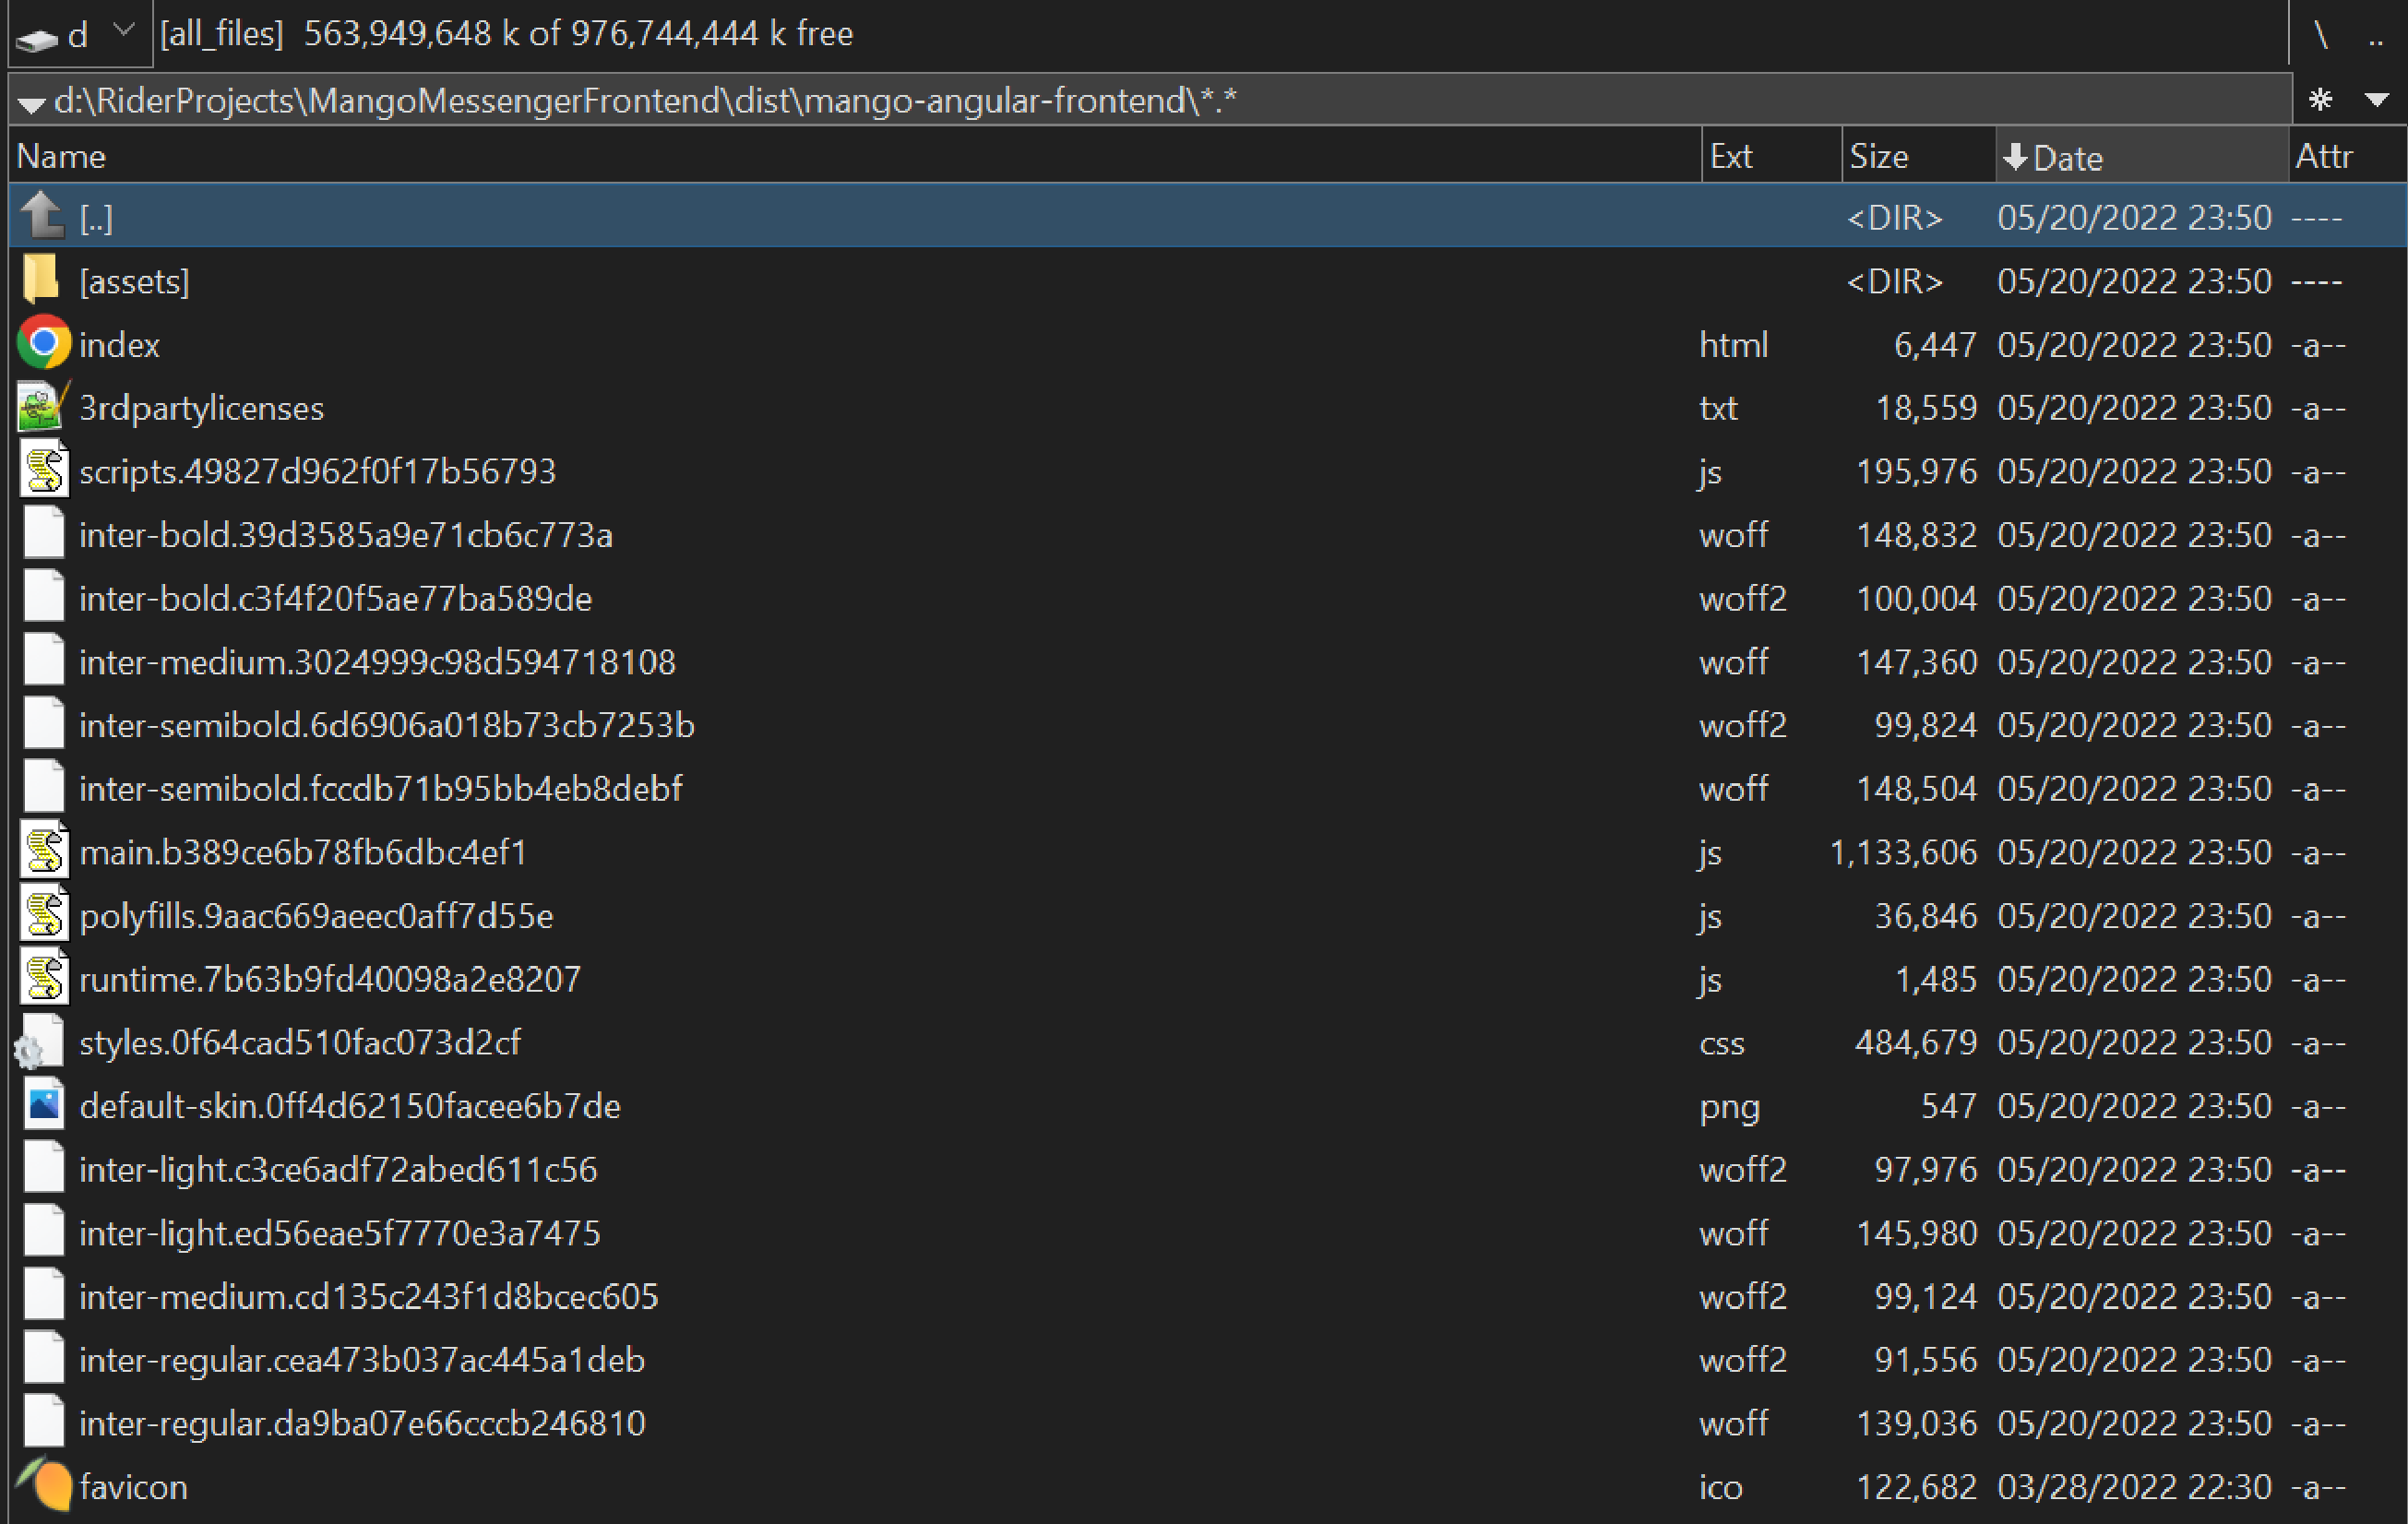
\includegraphics[width=1\textwidth]{img/08_build_angular_project}
    ~\caption{Dist folder containing angular build files.}\label{fig:figure24}
\end{figure}